349. Алексей, Борис, Виктор и Георгий играли в игры, ничьих не было. По итогам они частично заполнили таблицу, кто сколько раз у кого выиграл. Если в клетке на пересечении строки Алексея и столбца Виктора написано $2:1,$ это значит, что Алексей выиграл у Виктора 2 раза и 1 раз ему проиграл. Известно, что Георгий проиграл в три раза больше раз, чем выиграл; Борис выиграл пять раз; Виктор проиграл Георгию четверть от всех игр между ними; Алексей проиграл каждому одинаковое число раз. Сколько раз Алексей выиграл у Георгия? Заполните целиком таблицу ниже.\\
\begin{figure}[ht!]
\center{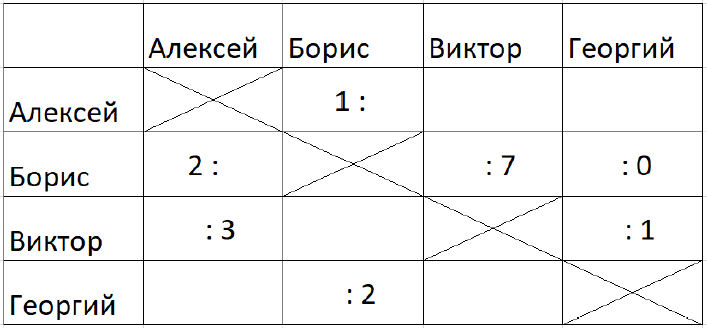
\includegraphics[scale=0.35]{tab3.png}}
\end{figure}\newpage\noindent
